% preamble
\documentclass[12pt, openany, a4paper]{book}
\usepackage[utf8]{inputenc}
\usepackage{graphicx}
\usepackage[a4paper]{geometry}
\usepackage{amsmath}
\usepackage{amssymb}
\usepackage{enumerate}
\usepackage[english]{babel}
\usepackage{titlesec}
\usepackage{sidecap}
\usepackage{caption}
\usepackage{subcaption}
\usepackage{glossaries}
\usepackage{float}
\usepackage{lipsum}  
\usepackage{listings}
\usepackage{setspace}

\usepackage[linesnumbered,ruled,vlined]{algorithm2e}
% \usepackage{gensymb}
\makeglossaries
\usepackage[numbers]{natbib}
% resources
\graphicspath{ {Images/} }
\setcounter{secnumdepth}{4}
\setlength{\parindent}{0em}
\setlength{\parskip}{10pt}
\renewcommand{\baselinestretch}{1.5}
\raggedbottom


\usepackage{color}
 
\definecolor{codegreen}{rgb}{0,0.6,0}
\definecolor{codegray}{rgb}{0.5,0.5,0.5}
\definecolor{codepurple}{rgb}{0.58,0,0.82}
\definecolor{backcolour}{rgb}{1,1,1}
 
\lstdefinestyle{mystyle}{
    backgroundcolor=\color{backcolour},   
    commentstyle=\color{codegreen},
    keywordstyle=\color{magenta},
    numberstyle=\tiny\color{codegray},
    stringstyle=\color{codepurple},
    basicstyle=\footnotesize,
    breakatwhitespace=false,         
    breaklines=true,                 
    captionpos=b,                    
    keepspaces=true,                 
    numbers=left,                    
    numbersep=5pt,                  
    showspaces=false,                
    showstringspaces=false,
    showtabs=false,                  
    tabsize=2
}
 
\lstset{style=mystyle}


\begin{document}
\frontmatter

%title page
\begin{titlepage}
\newgeometry{left=3cm, right=2.5cm, top=2cm, bottom=2cm}
\centering

%\includegraphics{UQ_Logo.png}\par
\vspace{4cm}
{\huge\bfseries Optimisation of Dragline Block Lengths \par}
\vspace{3cm}
{\Large\itshape Iain Rudge\par}
\vspace {5mm} 
{School of Mechanical Engineering \\ The University of Queensland\par}
\vfill
supervised by\\
Dr.~Michael \textsc{Kearney} (UQ)
\vfill
{\large \today\par}
\end{titlepage}
\restoregeometry


\cleardoublepage

% Letter to Head of School

% \begin{flushright}
% 	ADDRESS LINE 1\\
% 	ADDRESS LINE 2\\
% 	Tel.\ (07) nnnn nnnn\\
% 	\medskip
% 	\today
% \end{flushright}
\begin{flushleft}
  Dr. Ross McAree\\
  Head of School\\
  School of Mechanical Engineering\\
  The University of Queensland\\
  St Lucia, QLD 4072\\
  \bigskip\bigskip
  Dear Dr McAree,
\end{flushleft}

In accordance with the requirements of the degree of Bachelor of
Engineering in the division of 
Mechatronics

I present the
following thesis entitled ``Optimisation of Dragline Block Lengths''.  This work was performed  under the supervision of
Dr Michael Kearney  of the School of Mech Mining at UQ.

I declare that the work submitted in this thesis is my own, except as
acknowledged in the text and footnotes, and has not been previously
submitted for a degree at The University of Queensland or any other
institution.

\begin{flushright}
	Yours sincerely,\\
	\medskip
	\medskip
	\medskip
Iain Rudge
\end{flushright}

\cleardoublepage




\chapter{Acknowledgements}




\cleardoublepage

\chapter{Abstract}

% Notice that all \include files are chapters -- a logical division.
% But not all chapters are \include files; some chapters are short
% enough to be in-lined in the main file.


\singlespacing
\tableofcontents
\renewcommand{\baselinestretch}{1.5}

\listoffigures
\addcontentsline{toc}{chapter}{List of Figures}

\listoftables
\addcontentsline{toc}{chapter}{List of Tables}
\renewcommand{\baselinestretch}{1.5}
\onehalfspacing
% If file los.tex begins with ``\chapter{List of Symbols}'':
% \include{los}

\cleardoublepage

\mainmatter

	\begin{table}[h!]
	\centering
	\caption{Variables used in the report}
	\begin{tabular}{p{5cm} p{11cm}}
		\textbf{Variable Name} & \textbf{Variable Description}\\ \hline  \\ 
		Terra(x,y) & The function representing the height of the ground relative to a fixed point (x,y). It is assumed that this function will be a continuous function that is differentiable \\ \hline \\ 
		Coal(x,y) & A density function representing the density of coal prevalent in a point (x,y) in the mine. This function is not assumed to be continuous or differentiable, however will most likely be represented as a piecewise function.
		\\ \hline \\
		MaxBL & A constant, relating the maximum acceptable size of a block's length, this will be dependant on the draglines maximum reach and the movement patterns of the dragline.
		\\ \hline \\ 
		MaxBW &  A constant, relating the maximum acceptable size of a block's width, this will be dependant on the draglines maximum reach and the movement patterns of the dragline.
		\\ \hline \\ 
		MinBL &  A constant, relating the minimum acceptable size of a block's length, this will be dependant on the draglines maximum reach and the movement patterns of the dragline.
		\\ \hline \\  
		MinBW &  A constant, relating the minimum acceptable size of a block's width, this will be dependant on the draglines maximum reach and the movement patterns of the dragline. \\ \hline \\
		MineL & A constant that is the total length of the mine, it is a necessary variable as it will dictate one of the key constraints in the model. \\ \hline \\
		MineW & A constant that is the total width of the mine, it is a necessary variable as it will dictate one of the key constraints in the model.\\ \hline \\ Spoil(n,m) & This function is used to represent the amount of spoil generated by block (n,m). It can be stated that the function will be reliant on both Coal(x,y) and Terra(x,y). \\ \hline \\
		SpoilCap(n,m) & The amount of spoil that can be dumped into the exhausted block (n,m) this will be related in some manner to the amount of material removed from the block previously.
		\\
		\hline \\
		L(n,m) & The length of the nth block in the mth strip, this is one of the variables that our model aims to solve for. This is one of the outputs of the model \\ \hline \\ 
		W(n,m) & The width of the nth block in the mth strip, this is one of the variables that our model aims to solve for. This is one of the outputs of the model \\ \hline \\ 
		%		\[Spoil Capacity \in G,Dim\]
		\label{tab:var}
	\end{tabular}	
\end{table}
\newpage
\chapter{Introduction}
%!TEX root = ../main.tex
% state the general topic and give some background
% provide a review of the literature related to the topic
% define the terms and scope of the topic
% outline the current situation
% evaluate the current situation (advantages/ disadvantages) and identify the gap
% identify the importance of the proposed research
% state the research problem/ questions
% state the research aims and/or research objectives
% state the hypotheses
% outline the order of information in the thesis
% outline the methodology





% lets not go straight in with FPGA
% 
\section{Topic}
% The topic of this thesis is the mathematical modelling and optimisation of projected dragline mining by modelling the terrain of the strip as a density function. The projected planning of the dragline will aim to make use of minor simplifications or novel ways of modelling in order to create an efficient method for dragline excavation. This thesis does not explicitly intend to work with the software of others, however as explained in 1.1 a major point of this project is the ability to utilise the results of the thesis in other areas.
Draglines are massive machines used in open cut mining\cite{Bucyrus-Draglines}, weighing up to twelve tonnes \cite{DigBig} and with booms of up to 132.5 metres\cite{DigBig} these massive machines will move through a mine in a series of strips\cite{ORPlanning}. Each strip in a mine can be broken down into fundamental blocks which have an internal movement pattern\cite{A*Search}, depending on the machine the allowable sizes of these blocks will vary, as will the internal patterns. The purpose of this thesis is to develop a method of calculating block lengths for each strip in a mine such that if the time taken varies with the length of the block, then the minimal time spent per strip is found. However this method is not only useful for the calculation of an optimal path, the planning of blocks in a mine is an untapped topic of research, while products such as MineMax\cite{minemax} and polymathian\cite{polymathian} exist for pit mines and underground mines, no software packages exist for the planning and optimisation of a strip mine with regards to overburden removal with draglines.  While packages like those provided by Carlson mining solutions provide software capable of modelling a strip mine the algorithmic calculation of block dimensions within a strip is not considered. \cite{carlson} \\
As No methods exist in the space therefore the topic of strip generation in mining is valid for the exploration of throughout this thesis, while here only one strip is considered at a time the block dimension calculations are independent from strip to strip and as such will be able to be calculated as the mine is further explored. 


\section{Problem Definition}
% The problem at hand can be defined as the optimisation for the block sizing for draglines in a single strip. A one dimensional approach was taken for simplification of modelling and faster calculation time. The mine is modelled as a density function of the overburden to be removed and the remaining space within the spoil. Therefore a cost of block lengthn with regards to time must be found such that the overall cost of the strip can be found and optimised for. While no dragline is specified many are considered in this paper as a way to compare to results given from other papers. 
% \\
% More formally the problem can be defined as an optimisation problem to minimize time taken to mine an open cut strip using a dragline. This is acheived by varyin ghte length of the blocks within the strip such that the cost for each individual block is also minimized, for these reasons it is feasible to also model this as two intertwined optimisation problems. 
% % introduce research problem.
The aim of this thesis is the optimisation of dragline block lengths throughout a strip, where a block is the region of movement for a fixed movement pattern. While movement patterns that vary could be considered they are not within the scope of this project. The problem therefore can be defined as the calculation of feasible and optimal sequences of blocks within a strip. As no algorithmic methods exist for such a task the comparison and validation of results will be compared to examples from current pracetices in mining. Simply put the thesis is the minimization of time taken to remove overburden from a strip using a dragline. 



\section{Motivation}
The optimisation of strip mining within Australia has been the focus of many academic groups over decades of research \cite{DraglineDecade}. The reasoning for this is based firmly in economics. The majority of Australia's exports are derived from mining, with iron ores accounting for 20.2\% of Australian exports in 2014\cite{ExportStats} and coal accounting for an additional 11.6\% in the same year\cite{ExportStats}. These two industries alone accounted for \$104 007 million of national exports, \cite{ExportStats} which is a combined total of 32.8\% of the nations exports at the time. Therefore the core motivation for this project is to increase the efficiency of a dragline, as doing such will be financially beneficial,  it can be found that saving the industry 1\% of time will save \$35 million \cite{PacificCoal}.

Draglines are massive machines used in strip mining to remove overburden, allowing target minerals to be exposed and extracted\cite{IntoOpenPit}. Automating and optimising these procedures will lead to massive reductions in cost and time \cite{AutoEarthmoving}. The optimisation and automation of draglines has been a growing field. Initially the application of automation in draglines was seen as a challenging task, as the machinery must operate in harsh, complex three dimensional systems. \cite{IntroRobo}. In response to this challenge groups such as the 22 year old \cite{DraglineDecade} group, Shared Autonomy for Improving Mining Equipment Productivity, were formed to improve the autonomy and functionality of draglines.

The first attempts at automation were made in the 1980s \cite{CreativeEngineering}, the approach taken was to record the actions taken by an operator and then replay these actions in a loop. However this project was unsuccessful as the operator bases its movements on an instantaneous state\cite{CreativeEngineering} rather than just a goal state. This attempt at innovation however was not in vain as other faculties began investigating methods of automation in dragline mining.

In 1993, driven by previous work a model derived from vision-based robotic control \cite{VisionRobot}, was successfully implemented on a scaled model of a dragline. However, the methods of sensing and control initially provided difficulty in the application of this model to full scale machines \cite{DraglineDecade}. During this it was found that in a single cycle a dragline,  would spend 80\% of the cycle swinging in free space. \cite{DraglineDecade} This became the focus for many groups as it was seen as a potential area to reduce cycle time. The automation of a dragline and its components is a still developing field\cite{AutoEarthmoving}, however is not the main focus of this study. As the automation of draglines began to reduce the variance in operator it became apparent that other methods could be applied to optimise the motion and paths taken of the dragline.\cite{OperatorPerformance}. This research into path planning and modelling is a field that was and is still applied today. Topics such as motion planning, active control and path planning have all been applied to further improve performance in mining.\cite{DraglineDecade} In the year 2002 a two week test on a Bucyrus-Erie 1350 system showed that the machine was able to match or exceed the performance of an operator, a reduction in swing time was made and the system ran consistently at all points. \cite{DraglineDecade} This marked  an important step in the improvement of efficiency in draglines as it meant that additional modelling and path planning, as well as optimisation regarding movements could be considered with little to no operator variance\cite{IntroRobo}.

The motivation of this thesis is then in part based on the work of others in the automation of draglines, as it will allow former methods to be applied, and has allowed for more specific optimisations to be undertaken.In particular the optimisation of the movements of a dragline is a major task attempted to boost the efficiency of a mining system. Current models use a variety of methods, however the one that is of interest to this thesis is the use of mixed integer linear programming\cite{ORPlanning} in order to optimise the motions of a dragline. However with this application, as with other applications the run time of the simulation does not scale well. Therefore the motivation of this thesis is to determine an efficient technique that is capable of calculating the optimal lengths of blocks in a mining strip. These lengths can then be used in the previously stated models to increase runtime efficiency by reducing the amount of calculations required. 

In conclusion the motivation for this thesis is multi layered, at its core the main motivation is the financial benefit of optimisation in the utilisation of draglines, however many other researchers have been working on this task for decades, and as such any individual method is not feasible. Therefore this thesis seeks to help improve the runtime efficiency of current models by supplying a time efficient alternative in determining the optimal solutions for block size in conventional drag lines. 

% \section{Scope}

% \section{Assumptions}
% \section{Applications}

% \section{Research Goals}

\section{Thesis Structure}
\begin{description}
    \item[Introduction] Introduces the motivation and goals of the thesis while also properly defining the problem , variables and notation used throughout the thesis.
    \item[Background] A focused review of necessary information and background knowledge that is referenced and used throughout the thesis in the development of the algorithm, as well as methods and information that was considered throughout. 
    \item[Literature Review] A review of prior art and techniques that can be compared to the methods outlined in this thesis.
    \item[Design and Methodology] A systems level description of the design of the algorithm, including the assumptions and considerations made for each design choice.
    \item[Implementation] A detailed description of the implementation of each section, including discarded methods and results of the sections.
    \item[Results] Results of testing the software against prior art as well as results generated for the final strip mine,.
    \item[Discussion] A justification of assumptions and decisions made as well as a final comparison to other methods mentioned 
    \item[Conclusion] A summary of the thesis with a focus on the future of the project. 
\end{description}

\chapter{Background}
%!TEX root = ../main.tex
 \section{Mining Background}
Mining is a key part of this thesis, while not an in depth knowledge of mining is required, basic information is needed for problem definitions and clarity of communication. The focus of the thesis is the removal of overburden from strip mines using draglines, as this is a specific topic and not a general discussion on optimisation of mining machines in general only information on draglines and the environment in which they operate should be considered. Mining is a huge industry in Australia, making up 5.6\% of the nations GDP \cite{ExportStats} it is obvious that optimisation and planning is fitting in this field of industry\cite{DraglineDecade}.
However for mathematical models to be developed a thorough understanding of draglines should be gained to ensure the accuracy and validity of all formulated models. 
\subsection{Strip Mining}
Strip mining is the practice of removing a seam of material by removing strips of soil and overburden \cite{IntoOpenPit} to expose the underlying ore, this method is typically only viable near the surface, as a result some of the largest machines in the world are used in strip mining. Two techniques exist for the removal of overburden in strip mining \cite{Workpls} however here only the first will be considered. That is the flattening of an open area removal of overburden through strips. These strips span the length of the mine and will be removed sequentially, with the overburden from the current strip being dumped into emptied strips adjacent\cite{SMEBOOK}. Strip mining will recover a greater percentage of Ore and at a faster rate in comparison to underground methods \cite{SMEBOOK}, and as such is preferable when the appropriate conditions are met. Many machines are used in the process of strip mining, one in this process is the dragline which removes the overburden from a strip exposing the ore below\cite{IntoOpenPit}.
\subsection{Blocks}
A block is an element of  strip in which the dragline moves, these blocks make up a strip in an open cut mine. \cite{SMEBOOK} Draglines will not just move from the beginning of the strip to the end in a straight line, instead they move in patterns within the block \cite{IntoOpenPit}. This pattern is already the object of optimisation as the reduction of time spent within a block will itself reduce the total time taken to remove overburden from a strip. While the movement patterns within a block can vary from block to block it is assumed that they remain the same for this thesis. A block must be mined before all blocks after it. 
\begin{figure}[h]
\caption{Top down block view}
\label{blk}
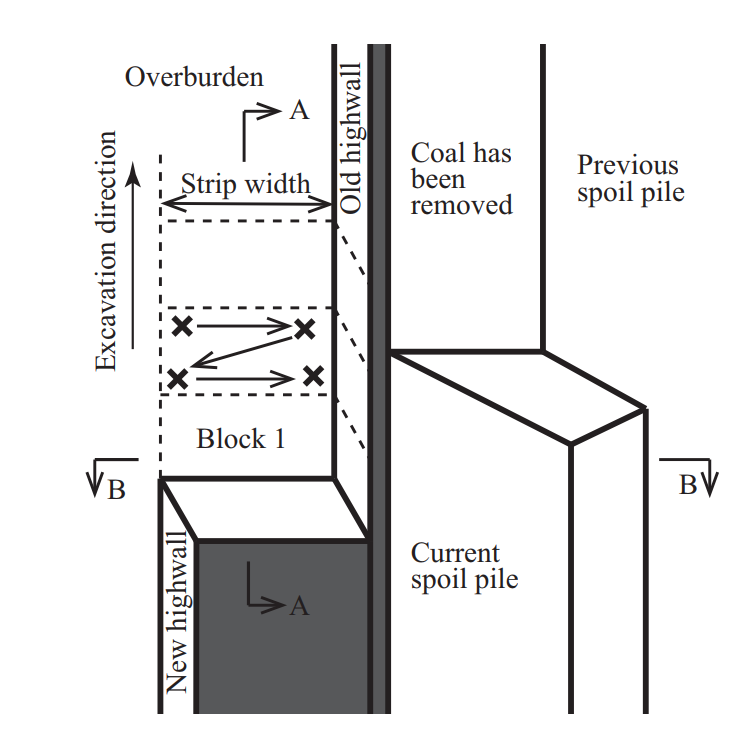
\includegraphics[width=\textwidth]{Block.png}
\end{figure}
\begin{figure}[h]
\caption{Side block view}
\label{blk}
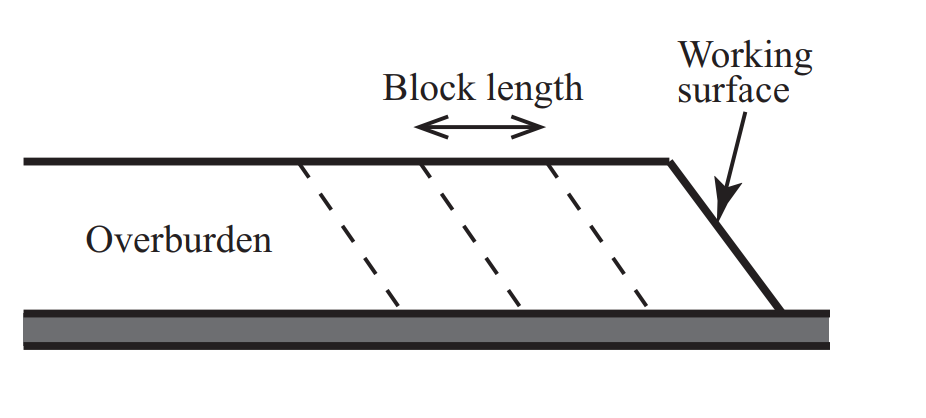
\includegraphics[width=\textwidth]{blockside.png}
\end{figure}

\subsection{Draglines}
A dragline is a massive machine used in open cut mining, working in strips to remove the overburden from a mine to expose the ore below\cite{ORPlanning}. The process that is done to achieve this is simple and cyclical in nature, first the bucked of the dragline is positioned above the material to be removed. Then it is lowered and pulled along the surface of the overburden, once the bucket is full it is lifted and moved above a spoil channel where it is deposited and the cycle is started again \cite{Dynamic Model}. The movement of a dragline may occur on two axis, a rotation or swing and a lift or hoist; these two actions convey the cost associated with using a dragline as they will typically be the only unique motions associated with both overburden removal and spoil dumping\cite{A*Search}. 


\section{Operations Research Background}
The field of operations research is a mathematical discipline specialising in the application of advanced analytical methods to make better decisions for specified problems \cite{Intro2or}. Often considered as a subsection of applied mathematics operations research employs techniques from mathematical modelling and optimization theory to calculate optimal or near optimal solutions to complex decision making problems\cite{abtOR} \\ Naturally this branch of mathematics lends itself to the problem of optimal block dimensions in a strip mine, with the use of optimal decisions through either precise calculation or policy the best possible solution can be found using the field of operations research. The scope of this field is diverse, with many potential solutions to a problem. As such the selection of mathematical modelling and optimisation techniques should be considered carefully to result in an accurate solution. 
\\
Mathematical modelling is a vital section of operations research, however the problem can be written and formulated in many different ways, as such the specific formulation styles of a technique will also be mentioned in that section, modelling in general can follow some simple rules yet no overall method or technique exists for the creation of a mathematical model, it is instead reliant on understanding of the system. 

\subsection{Linear Programming}
Linear programming is a technique used to obtain the optimal outcome of a model such as the minimal time or highest profit\cite{LPII}. This method can only be applied to a mathematical model with a linear objective function subject to linear equality and linear inequality constraints\cite{Intro2or}.\\ Often the model is described as groups of variables and constraints with an overall objective function. This method of optimisation is often solved using complex optimisation engines such as gurobi rather than through algorithms implemented specifically for the implementation. The process of optimisation is done by defining a feasible region of valid solutions as a convex $n^{th}$ dimensional polytope, where $n$ is the dimensionality of the variables associated\cite{oriNTRO}. Here this polytope is defined as an intersection of a finite amount of half spaces defined by linear inequalities. Within this polytope the optimal feasible solution will be found on a vertex satisfying all constraints and the objective function, this method can be calculated using matrix manipulation in algorithms such as the modified simplex algorithm\cite{LP}.  	
\\
The standard variables in a linear program are continuous, however a sub technique of linear programming is integer programming which adds the constraint that some variables must be full positive integers \cite{LPII}. This problem is typically harder to solve as the optimal linear solution may not be similar to the optimal integer solution\cite{Intro2or}. An integer solution is often calculated by calculating an optimal linear solution and branching on rounding decisions \cite{LPII} for the integer variables to create a decision tree. This tree is branched such that the difference between the linear solution and chosen integer solution is minimised, this is the origin of the increased difficulty of integer programming in comparison to linear programming\cite{oriNTRO}. 

\subsection{Dynamic Programming} 
Dynamic programming is a method of optimisation in which a sub-problem is solved and the solution stored \cite{Bellman}, this is done for all sub-problems until the full problem can be constructed from, if a sub-problem has already been solved and stored then it is called from memory instead of through calculation \cite{MITDynamic}. The process of storing sub problems for later use is called memotisation\cite{Bellman} and is vital for use in dynamic programming as dynamic programming often encounters similar sub-problems when working recursively\cite{MITDynamic}. \\

Typically a dynamic program refers to recursively breaking down decisions into steps through a stage \cite{DPfound}. The value of each decision in a stage is a combination of the initial myopic value of the choice as well as the value of all other solutions that occur after this decision is made\cite{DPfound}. This requires that some state in the problem is altered when a decision is made, then the affects of this decision must also be considered for all subsequent choices. This creates and expanding tree of subproblems and is why the method of memotisation is so vital to dynamic programming as often the same sub-problem will be encountered multiple times\cite{Bellman}. 
\subsection{Metahueristics} %Should I mention this if I looked into it but never used it
A metahueristic is a higher level optimisation technique used to find, generate or select a heuristic that may provide a good solution to an optimisation problem\cite{Meta}, typically when working with incomplete information , inaccurate information or limited computational power\cite{Meta}. Unlike Linear programming and dynamic progamming a metahueristic does not garuntee a globally optimal solution , due to metahueristics typically relying on stochastic optimisation to generate solutions. \\
The genetic algorithm is such an example of a metahueristic where candidate solutions are evolved to find a better solution\cite{GA}, this is done by calculating the value of all candidates. After this is complete the more preferable solutions are combined with one another in such a way that a new series of candidate solutions is generated \cite{GA}. This is done iteratively until the change between generations is sufficiently small, at this point either a local optimal or global optimal solution can be found. Typically the genetic algorithm is used for determining a policy for good solutions, rather than linear programming or dynamic programming which will calculate the true optimal solution. 


\chapter{Literature Review}
%!TEX root = ../main.tex
\section{Mining Background}
\subsection{Strip Mining}
\subsection{Draglines}
\subsection{Blocks}

\section{Operations Research Background}
The field of operations research is a mathematical discipline specailising in the application of advanced analytical methods to make better decisions for specified problems. Often considered as a subsection of applied mathmatics operations research employs techniques from mathmatical modelling and optimization theory to calculate optimal or near optimal solutions to complex decision making problems. \\ Naturally this branch of mathematics lends itself to the problem of optimal block dimensions in a strip mine, with the use of optimal decisions through either precise calculation or policy the best possible solution can be found using the field of operations research. The scope of this field is diverse, with many potential solutions to a problem, however the generation of the matematical model will aid in selecting a method that will obtain results quickest. \newline
Mathematical modelling is a vital section of operations research, however the problem can be written and formulated in many different ways, as such the specific formulation styles of a technique will also be mentioned in that section, modelling in general can follow some simple rules yet no overall method or technique exists for the creation of a mathematical model, it is instead reliant on understanding of the system. 

\subsection{Linear Programming}
Linear programming is a technique used to obtain the optimal outcome of a model such as the minimal time or highest profit. This method can only be aplied to a mathematical model with a linear objective function subject to linear equality and linear inequalitiy constrants.\\ Often the model is described as groups of variables and contstraints with an overall objective function. 	
\subsubsection{Linear Programming}
\subsubsection{Presolving}
\subsubsection{Integer Programming}
\subsubsection{Mixed Integer Programming} %Mentioned as a potential solution and was tested 

\subsection{Dynamic Programming} %Used in final code 
\subsection{Metaheuristics} %Should I mention this if I looked into it but never used it
\subsubsection{Approximate Dynamic Programming}
\subsubsection{Genetic Algorithm}


\chapter{Design and methodology}
%!TEX root = ../main.tex

\section{Modelling Data}
The modelling of data in this thesis is the vital first step to the optimization of a dragline, any simplifications made in this step will carry through all steps of the algorithm and effect the accuracy of the final results, therefore the manipulation of data to suit the system must be considered very carefully. As the dimensionality of the data decreases the runtime will as well, however the acheivable accuracy will decrease as the system will become more general. The method selected for the modelling of the geological data is a one dimensional density function used to represent the amount of overburden required to be removed from the mine along a specific strip. While this is not ideal in terms of a truly optimal solution it will allow the program to run rapidly, many assumptions along the way will result in loss of optimality at many stages, while an optimal solution is the desired result any feasible or near optimal solution is also acceptable. 
\\
Alternate methods that were considered for the modelling where a data driven approach or a two dimensional aproach, while a data driven aproach lends itself to machine learning of meta hueristics, these methods are often slow and not garunteed to lead to an optimal solution 
\\

One dimensional density functions are also useful as they can be generated through many methods, either through a pregenerated mine for testing or through geological survey data. In the thesis the sample data was generated by generating typical mine shapes and layouts of interest, such as a ramp and step function; within these samples a noise function was applied to give a better and more realistic set of data to test on. Survey data was supplied in a .xyz format, by assuming a constant depth of cut and a homogenius density of overburden the one dimensional density function was taken along the centre of the proposed strip path. This density data was represented as an Linked list for ease of use in python, an additional reason for this decisionis that the mine will always be mined in order and as such the list will simply be traveresed from start to end.  


\subsection{Types of Input}
The intended use of the program is to rapidly calculate optimal, near optimal or feasible block dimensions fora single strip inside a mine, however one of the key features of the program is its relaticly rapid runtimes, allowing on the fly adjustments and the ability to make corrections and compensations for errors. This input however is harder to predict and could be considered outside the scope of the project. As the thesis focuses more on the algorithms and underlying princples of the software rather than the user interface and user experience it is considered that the input to the project is a 1 dimensional array representing the spoil and another representing the mine at the current point in time, this will allow for expansion if required for on the fly adjustments. The program can also have the specifics of the dragline changed so that any possible dragline can be considered, while this is simple to change there is no user interface for the program and as such if it were to see further use then a graphc user interface would need to be constructed. \\

\subsection{Assumptions}

\section{Cost of Overburden Movement}
The cost of a block is vital to the solution to the problem, however the cost of a block is calculated as a summation of many individual movements, therefore the proper consideration for these models should be undertaken, ideally the cost of overburden movement will be able to calculate the time of movement for the action of moving overburden from point $n$ in the mine to $s$ in the spoil strip. Therefore two inputs would be the only required information for this function.
\subsection{Scope}
The function to calculate the cost of an action is required to work for all $n\in N , s \in S$ if this movement is at all valid, therefore we can assume that only valid enteries will be passed into this solution. Therefore for any valid combination the function should return a cost of movement, while the cost funtion is not required to be linear it must be able to be used in a Linear programming engine such as Gurboi, and as such must be Linearly related to block usage for objective funtions. This is the most pressing constraint as otherwise linear programming will be infeasible.
\subsection{Assumptions}
\subsection{Justification}

\section{Cost of a Block}
\subsection{Scope}
\subsection{Assumptions}
\subsection{Justification}

\section{Cost of a Strip}
\subsection{Scope}
\subsection{Assumptions}
\subsection{Justification}

\section{Communication of Results}
\subsection{Scope}
\subsection{Assumptions}
\subsection{Demonstration}

\chapter{Implementation}
%!TEX root = ../main.tex

%FLUFF THE INTRO
\section{Modelling}
Modelling of a real world system has two motivators, the first is to gather better understanding of the system through mathematics and data analysis, the other is to allow operations such as optimisation and simulation onto the system. However there are challenges that can affect the accuracy of the model, as such careful deliberation should be taken to make good assumptions and simplifications. The assumptions and simplifications that are made will be explained and justified for each relevant algorithm, sub-model and constraint; all of which are needed to properly communicate the model in such a way that is independant of the optimisation techniques used.  
\\
The models defined in this section of the report will be used in all optimisation methods attempted, the accuracy of these models is vital to the accuracy of any formulation dependant on them and as such proper considerations and justifications must be made. The models that are discussed here are inherine to the system, they are often constants or functions within larger problem formulations, as such they are simple to change but yet key to the accuracy of the thesis. \\
The models discussed here are broken into four major sections, proper modelling of spoil distrobution, modelling of movement patterns within a block, modelling of data unique to a dragline and finally the modelling of an action. Each of these catagories aligns with a specific section of a formualtion, and as such can be developed indepentandly of each other. 
\subsection{Spoil modelling}
The Spoil or overburden is the strictest constraint on the feasblitly of a strip, as such the modelling of spoil distrobution is vital to the accuracy of a model. The spoil channel can be discretised into sections with a given maximum capacity per section, following this the swell rate of the spoil and expansion factor due to ineffcient spoil placement should also be considered. These three models are the required knowledge to properly consider and implement spoil capacity constraints on a formulation, each model can be seen below. 
\subsubsection{Spoil Capacity}
The capacity of a section of spoil is a vital constraint in the formulation of a block model
\subsubsection{Swell Factor}
\subsubsection{Spoil Expansion Factor}
\subsection{Movement through a Block}

	
\subsection{Dragline Dynamics}

\subsection{Action Cost}

\section{Optimisation at the Block Level}
In order to model a sequence of blocks it is vital to first develop an accurate model describing the cost and spoil of a block, several methods were considered, each of which was an optimisation problem seeking to minimise the time taken to process the block. The calculation and modelling of a block must be rapid, as this modelling function will be used thousands of times in the calculation of a strip, while storing block costs into memory was originally considered the feasability and cost of a block varies with three inputs, its start and end locations, and the curent state of the spoil. Therefore the amount of unique blocks that can be considered is huge and storing results in memory loses effciency. \\A variety of methods were formulated and the results were compared against one another for both run time and accuracy, in order to verify the accuracy of a model its output is compared to techniques that are outlined in sections \ref{PA:MIP}, \ref{PA:DP} and \ref{PA:GA}. This comparison was done on both real world data and standard data sets that were generated for the purpose of testing. The comparison will focus on the run times of each solution as well as the accuracy of the method proposed. 

\subsection{Mixed Integer Programming}
Mixed Integer Programming is a somewhat obvious choice for this model, as this technique is already applied in a 3 dimensional enviroment as outlined in section\ref{PA:MIP}, however some changes must be made for this model to be used with the modified density data, as a result while the concept of a MIP was still considered, the problem itself had to be reformulated. Formulation for the model is found in the following section, while developing a MIP it is vital that all constraints and objectives are lineary related to data and variables, otherwise the solver algorithms will not work. The prcess of formulating an approporate model for the block cost is based on the physical movements of a dragline and the constraints that will affect it, while some elements of the formulation were adjusted or ignored, the end formulation is the most accurate model with the data available. 
\subsubsection{Model Formulation} 
\paragraph*{Sets}
\begin{align}
\label{MIP:Set:S}
S\qquad \text{Set of all Spoil Sections   } s\in S\\
\label{MIP:Set:N}
N\qquad \text{Set  of all Mine Sections } m \in M
\end{align}
Here the sets are used to represent the discretised mine and spoil sections, while these sets have no effect on the system they are used for ommunication of data and variables. The sizes of sets $S$ and $M$ must be the same as the spoil channel is the results of a prior strip in a mine. The discretisation of the Mine into sections was chosen as the move from a continues model to a discrete model made the modelling of the problem much easier. While some information is lost in this process it is negligible as survey data itself is discrete. The size of the sections themselves are dependant on both survey data and desired accuracy, for the testing of this thesis each section was a metre in length, however if more precision is required then the resoltion could be increased. However the increase in detail and resolution will result in slower calculations of block dimensions as more potential solutions are presented. One metre was selected because it was the resolution of the real world data supplied however as seen in the comparison of results a lower resolution will dramatically speed up the run time of the problem, this could be used in first pass solutions to get an approximation of good results. 
\paragraph*{Data}
\begin{align}
\label{MIP:Data:SF}
SF \qquad \text{Swell Factor of Spoil}\\
\label{MIP:Data:Seff}
SEf \qquad \text{Packing Efficiency of Overburden}\\
\label{MIP:Data:SpoilCap}
SpoilCap \qquad \text{Maximum capacity of spoil}\\
\label{MIP:Data:n}
n_{j} \qquad \text{Density of overburden at section $j$} \quad \forall m_{j}  \in M\\
\label{MIP:Data:s}
s_{j} \qquad \text{Density of overburden at section $j$} \quad \forall s_{j}  \in S\\
\label{MIP:Cost}
C_{jk} \qquad \text{Cost of movement from $m_{j}$ to $s_k$ }\\
\label{MIPDvol}
Dvol \qquad \text{Volume of overburden moved in one action}
\end{align}
The data relevant to the formulation of the MIP is modelled and calculated in section 4.1, in this section models and justifications can be made for each design choice that is made in the accuracy of the data however in this section the way that the data is used is much more important. The data used is relativly simple, often represented as either a constant or an array of constants. The use of data \ref{MIP:Data:SF} to represent the swell of spoil is vital to the proper modelling of spoil distrobution and will be used whenever interacting with the spoil output of the system, this data is simply a constant value, as suggested in the prior section. Similarly data from \ref{MIP:Data:Seff} is used as a n approximate model for teh expansion of the spoil due to ineffciencies in stacking methods, this constant can vary depending on the model used however is simply represented in the formulation of this problem and is not a key data point for intial testing, rather it is important for the accuracy of the spoil channel distrobution, which itself is also dependant on data \ref{MIP:Data:SpoilCap} or the maximum capacity of the spoil at any given section $s$, here we assums that this capacity is constant throughout the spoil chanel, however this could be easily adapted if needed for varying capacities. This capacity is used in constraint \ref{MIP:SPcap} as the right hand side of the equation. Sensitivity analysis could be done on this constraint to estimate the potential benifits of increasing the capacity of spoil available, this would have the same effect as increasing the effciency of the spoil stacking methods, as described by a lower value of data\ref{MIP:Data:Seff}.\\
The amount of material moved per action can be found in data \ref{MIPDvol}, while a very simplistic peince of information it is still necissarry to include as it represents the amount of overburden moved per action through the size of the draglines bucket. Sensitivity analysis could also be done to relate how the changing size of this constant affects the mining time of a block, icreasing this constraint should reduce the cost of the block as it will reduce the amount of actions required to remove the overburden from a mine section. This cost is found in data \ref{MIP:Cost}however this data is an $m\times s$ array that contains the movement cost from each point $m\in M$ to each spoil section $s \in S$, the movement cost is used in the objective function to minimize the total swingtime of the dragline inside a block. This cost data can be calculated as a function $\arctan(\frac{abs(n-s)}{Reach})$ however this may also be precalculated and put into an array to reduce function calls, the latter method was selected for the implementation of this data. 
\\
The representation of the mine\ref{MIP:Data:n} is an $1\times m$ array where the value at each point is the average amount of overburden to be removed at that point, this value will not change as we will never come back to or refer to a sectiononce the overburden has been removed. Unlike this is data \ref{MIP:Data:s} which represents the amount of overburden currently in the spoil. Once a block is calclulated this spoil value is updated so that future blocks use the spoil ouput of the previous block to hae a consistent and proper model for the spoil distrobution throughout the strip. Therefore while this data will not change during the calculations performed on the block, once the solution is calculated this data is updated to reflect on the resultant spoil. 
\paragraph*{Variables}
\begin{align}
\label{MIP:M2S}
X_{jk} \qquad \text{Overburden moved from $m_{j}$ to $s_k$ }\\
\label{MIP:MCeil}
Y_{jk} \qquad \text{Actions moving from $m_{j}$ to $s_k$ }
\end{align}
The variabes for this model are both related to the movement of overburden from a moint $m$ in the mine to a point $s$ in the spoil. Variable \ref{MIP:M2S} refers to the capcaity of dragline volume that is moved from $m$ to $s$. This is necissary for the calculation of spoil capacity constraints as well as the calculation of removal of overburden from the mine at point $m$. However the assumption is made that movement actions taken at any capacity will still incure the same costs. It is for this reason that variable \ref{MIP:MCeil} is used, representing the ceiling of actions taken from point $m$ to point $s$ for all points in the mine. This variable is exsclusvly used in the objective function, participating only in constraints that allow it to be linked to \ref{MIP:M2S}.
\paragraph*{Objective}
\begin{align}
\label{MIP:OBJ}
\min\left(\sum_{m\in M}\sum_{s\in S} (C_{n,s}\times Y_{n,s})\right)
\end{align}
The objective function of the Mixed integer linear program is simple, the minimisation of time taken to complete all actions. As some actions will cost more than others it becomes obvious that the cheapest possible movement will be selected when available, it should be noted that while cost\ref{MIP:Cost} is not linear, its relationship with movement actions \ref{MIP:MCeil} is, allowing linar programming to be used. The minimization of this is obvious, as smaller movement actions will take less time than a larger swing action, they will be preffered where feasible. 
\paragraph*{Constraints}
\begin{align}
\label{MIP:RemoveAll}
\sum_{s}X_{m,s}\times Dvol = M_{m}  \quad \forall m\in M  \\
\label{MIP:SPcap}
\sum_{m\in M} X_{m,s}\times SEf \times SF + S_s\leq SpoilCap \quad \forall s \in S \\ 
\label{MIP:Link}
X_{m,s} \leq Y_{\mu,s} \quad \forall m,s \in M,S\\
\label{MIP:Housekeeping}
X_{m,s} \geq 0 \qquad \forall m \in M , s \in S\\
Y_{m,s} \in \mathbb{N} \qquad \forall m \in M , s \in S
\end{align}
The constraints on the model could be considered as the most interesting part of the model, with no constraints the model would simply choose to perform no actions, as this is the minimal allowable solution. Therefore the minimum amount of work done by the dragline must be constrained, the strict constraint fouun in  equation \ref{MIP:RemoveAll} states that all overburden must be removed from a section $m$ for all sections in the mine. The purpose of this constraint is to set the exact amount of work done by the dragline, it must remove all overburden from the block, but cannot remove any additional material from the block, while the latter is less likely as this would increase the cost of operation it is still best to have as strict a constraint as possible. \\
The constraint described in equaion \ref{MIP:SPcap} constrains the solution the most of any constraint in not only the Block model but the entire thesis, it is the feasability constraint that the spoil capacity cannot be exceeded, it should be noted that this constraint also takes into account the state of the spoi prior to this block, allowing past blocks actions to carry over. This constraint will invalidate many solutions and cause the cost of action to go up if all local spoil sections are at or close to capacity, this constraint is what drives up the cost in the calculation of a block. 
\\ Constraint \ref{MIP:Link} is the linking constraint between $X$\ref{MIP:M2S} and $Y$\ref{MIP:MCeil}, it ensures that $Y$ is the cieling of $X$. As the objective is a minimisation problem, then $Y$ will seek to be the lowest allowable integer value greater than or equal to $X$, this linking constraint ties constraints \ref{MIP:RemoveAll} and \ref{MIP:SPcap} which are both dependant on $X$ to the objective function \ref{MIP:OBJ} which is dependant on $Y$. Similarly constraints \ref{MIP:Housekeeping} simply state that $X$ must be a positive real number and $Y$ must be an integer greater than or equal to zero, these constraints are simply to properly set up the variables for the model. 
\subsubsection{Implementation}
[Put Code Here]
\begin{lstlisting}[language=Python]
		m = G.Model()
		X = {(n,s):m.addVar() for n in self.N for s in self.S}
		Y = {(n,s):m.addVar(vtype = G.GRB.INTEGER) for n in self.N for s in self.S}
		m.setObjective(G.quicksum((self.MoveCost(n,s)*Y[n,s]) for n in self.N for s in self.S),G.GRB.MINIMIZE)

		CreateCieling = {(n,s):X[n,s]<=Y[n,s] for n in self.N for s in self.S}

		RemoveOnlyallowed = {
		(n):m.addConstr(G.quicksum(X[n,s]*self.Dragline.get_BucketVol() for s in self.S)==self.Mine[n]) for n in self.N
		}

		spoilcapacity = {
		(s):m.addConstr(G.quicksum(X[n,s]*self.Dragline.get_BucketVol()*self.swell*self.expand for n in self.N)+self.Spoil[s]<=self.spoilcap)
		for s in self.S
		}

		m.optimize()
\end{lstlisting}
The implementation of the model is done in python, with use of the gurobi optimisation engine linear programming becomes a very simple method. Lines 2 and 3 are the decleration of variables relating to the variables found at equations \ref{MIP:M2S}, \ref{MIP:MCeil} corresponding to them exactly. From here the objective is declared and set to minimise , matching the objective \ref{MIP:OBJ} stated in the formulation section. The constraints are also similar with each constraint \ref{MIP:Link},\ref{MIP:SPcap},\ref{MIP:RemoveAll} all represented in code. For additional information on supporting code please refer to Appendix A. Once the formulation is complete gurobi will perform preprocessing on a matrix representation of the model, before using the modified simplex algorithm to solve the linear problem, while this algorithm could be written specifically for this thesis it was seen as unecissary as the gurobi optimisation engine is much more effcient at this task. 
\\
Once this optimisation algorithm has been completed the spoil is updated and the cost is returned, this is done by simply updating the relevant sections of the array and can be seen completed in the below code snippet.
\begin{lstlisting}[language=python]
self.cost = m.ObjVal
self.potential_spoil = self.Spoil[:self.stemp]+[sum(M2S[n,s].x*\
self.Dragline.get_BucketVol()*self.swell*self.expand for n in self.N)+self.Spoil[s]\
 for s in self.S]+self.Spoil[self.etemp:]

\end{lstlisting}
This entire process is then wrapped into one fucntion so that the cost of a block can be calculated though one function call, vital to the application of this model in the optimisation of the entire strip. 
\begin{lstlisting}[language=python]
	def BlockCost(self,start,end,Spoil,output=0):
		if end>len(self.Mine):
			end = len(self.Mine)
			# print("Adjusting End Position")
		self.set_Spoil(Spoil)
		if output ==1:
			print("Spoil Set")
		self.set_Block(start, end)
		if output ==1:
			print("Block Set:\t" ,[start,end])
		self.Calc_Valid()
		if output ==1:
			print("Column Generation Done")
		stime = time.time()
		try:
			self.MIP(output)
			etime = time.time()-stime

		except:
			etime = time.time()-stime
			print('\t MIP Infeasible')

			return(np.inf,Spoil,etime)
		if output ==1:
			print("MIP Complete")
		return (self.cost,self.potential_spoil,etime)
		\end{lstlisting}
The only unique or interesting part of this function is that if the block is not feasible then the function will return a cost of infinity, this will mean that the block will not be used in the optimal or feasible soluion of a sequence of blocks in a strip. Each call of the function take in the start, end and state of the spoil, allowing the block to be calculated to return the cost and updated spoil, as well as the time taken to calculate the MIP. Both cost and resulting spoil are vital to the calculation of the strip, and are the two desired outputs of any model describing the actions taken within a block. 
\subsubsection{Results}
\subsection{Mixed Integer Programming with Validity}
This model is an updated version of the Mixed Integer model with only one added array of data and one additional constraing, however this single constraint makes a huge differences to the complexity and accuracy of the model. The constraint that a dragline cannot move to or reach every point in a block or in the spoil will constraint the areas where overburden can be distributed in the spoil section. This constraint was not intially obvious as typically the dragline will place spoil in local areas rather than in sections that would be out of its reach. However as the availability of spoil room is reduced the cost assocaiated with this action is seen as prefferable rather than an infeasible solution. This was only found after an implementation of the strip optimisation was complete, and as such can be seen as an updated model. 
\subsubsection{Model Formulation}
\paragraph*{Additional Data}

\begin{align}
\label{MIP:Data Valid}
Z_{jk}  = \begin{cases} 1& \text{if movement from $n$ to $s$ is valid}\\
0 & \text{Otherwise}   \end{cases} 
\quad \forall n \in N s\in S
\end{align}
This data is an $m\times s$ array of binary values, such that if the dragline is ableto feasibly reach the section of spoil when mining the section $m$ of overburden then the arrays value is 1 and 0 otherwise. This array is currently based on the feasible  maximum and minimum reach of the dragline, however other factors such as the pit edge while starting a new block, or having to move over sections in the spoil may cause this array to become more complex. Updating and improving this data should be of high importance for an accurate model, however as it is not integral to how the algorithm works, some simplifications can be made.
\paragraph*{Additional Constraints}
\begin{align}
\label{MIP:Valid}
Y_{n,s}\leq \infty\times Z_{n,s} \qquad \forall n \in N , s\in S
\end{align}
This constraint is a big M constraint, that is it will limit the value of Y unless the value of Z is one for that combination of m and s. This constraint is simply implemented and constrinct the feasible solutions of the model, it should be noted that this is setting most of the potential values of Y and X before any optimisation is considred, doing this has a dramatic effect on the reduction of runtime. As less options are available, less calculations mustbe considered and as such the program can run faster.
\subsubsection{Implementation}
The code for this section is the exact same as previously, however one additional constraint is added, as can be seen below it is very simple to add additional contstraints into the gurobi model.
\begin{lstlisting}[language=python]

OnlyifValid = {
		(n,s):m.addConstr(Y[n,s]<= np.inf*self.isValid[n-self.start,s-self.start-self.Dragline.get_reach()]) for n in self.N for s in self.S
		}
\end{lstlisting}
However more interestingly is the calculation of valid blocks, as mentioned previously, the simplistic model for a valid block is if it is within the reach of the dragline, while this is not an accurate model it is suffcient for the demonstration of the block planning algorithm and with more time could be developed to be more fitting for application. 
\begin{lstlisting}[language = python]
def Calc_Valid(self):
	self.isValid = np.zeros((self.end-self.start+1,self.end-self.start+2*self.Dragline.get_reach()+1))
	for i in range(self.end-self.start):
		for j in range(i-self.Dragline.get_reach(),i+self.Dragline.get_reach()):
			self.isValid[i,j+self.Dragline.get_reach()] = 1
\end{lstlisting}
Here the array size is set up, we only consider areas within the block and spoil and as such this will reduce the size of the array and allow for more rapid calculation of results. Once this is done for every possible combination of blocks in this window a check is done to ensure that it is a valid movement. 
\subsubsection{Results}


\subsection{Dynammic Programming}
Dynammic programming is another potent
\subsubsection{Model Formulation}
\paragraph*{States}
\begin{align}
\label{Stte}
S \quad \text{State of spoil at current stage}
\end{align}
The state of a formulation is the current resources of remaining in a resource constrained dynammic program. Here this is the spoil channel, which will change with every action and therefore is updated at every stage, this state alongside the current stage should be stored in the memory so that the process of memotisation can occur. This technique uses the princeple of optimality to reduce the amount of calcualtions required, that is if we have already calculated the optimal path for the block from this stage with the current states then the solution is already known and that branch of exploration can be completed. However the only state in this formulation is the amount of spoil in each section at the current stage, the use of this state is vital as it is used for the constraint on the actions available at each point. The spoil is a state as it will change with each action, nothing else will change depending on the action taken and therefore all other dynammic variables are simply stages. 
\paragraph*{Stages}
\begin{align}
\label{DP:Stage0}
H \quad \text{Overburden remaining at current block}\\
\label{DP:Stage1}
M \quad \text{current mine section }m \\ 
\label{DP:stage2}
D \quad \text{Position Of Dragline}
\end{align}
The stages of the model are something that we do not have control over, each action moves us from one stage to the next. This formulations two stages are interlinked, however it could also be seen that the position of the dragline is dependant on the current mine section. Therefore the model has effectivly two stages, the overburden left at the current section and the current section within the mine. Once all overburden is removed from the stage $H$ the position $M$ is updated. If the position is suffciently updated then the draglines position also will update. For any given block these stages will occur in the same order no matter what. This is the differentiation between states and stages, the dragline will always move through the block and remove all overburden however the actions taken to remove the overburden will not always be the same. Here the states are selected as the minimum required representation of the block in order to properly model its behaviors and movement process. 	
\paragraph*{Transistion Function}
\begin{align}
\label{Transition}
S_{stage+1}(s)=S_{stage+1}(s)\times SEf  \text{where $s$ is the spoil section in action }
\end{align}
The transition value allows the next state to be calculated based on the current state and the action chosen. Here the action chosen is the movment of overburden from the current block to some point on the spoil $s$, this action will succeed in adding additonal overburden to the relevant section on the spoil, updating this is simple and from here the only additional peice of information required is the constraint that this tranistion fucntion cannot create a state that exceeds the spoil capacity, this is done by simply checking the suggested next state and adding a large cost if this constraint is violated. 
\paragraph*{Value Function}
\begin{align}
\label{value}
C_A = \arctan(\frac{abs(D-A)}{Reach})\\
V_t(S_t) = \min (C_A+V_t(S_{t+A}))
\end{align}
The value function calculates the cost associated with agiven action based on the cost of the action and the resulting states for all future stages, the cost of an action is simply the swingtime from the current block to the spoil selected as an action. This cost is to be minimised however will also affect the state of the next action, as such this will recursivley consider all potential courses of action for each action taken. Therefore teh more actions that can be made the more computation time is required to calculate the cost of a block. 
\subsubsection{Implementation}
\begin{lstlisting}[language=python]
_Bucket ={}
M = MineGen(100)
S = [0 for i in range(130)]

def Bucket(Cur,End,SP,M,Scoops,H,D-):
    global _Bucket
    SPtup = str(SP)
    SPmax = 150
    Reach = range(D-20,D+20) 
    if D < 20:
        Reach=range(0,D+20) 
    if D-Cur<=5:
        D = D+5
    if H <=0:
        Cur = Cur+1
        Scoops = 0
        H = M[Cur]
    if Cur == End:
        return (0,0,0,0,[],0)
    if (Cur,End,Scoops,SPtup) not in _Bucket:
        _Bucket[Cur,End,Scoops,SPtup] = min((costspoilNL(Cur,A,H,D)+
            Bucket(Cur,End,SP[:A]+[SP[A]+28]+SP[A+1:],M,Scoops+1,H-10,D)[0],Cur\
                  ,A,Scoops,SP[:A]+[SP[A]+28]+SP[A+1:],D)for A in Reach if\
    SP[A]+28 <= SPmax)
    return _Bucket[Cur,End,Scoops,SPtup]

def GetData(Start,End,Mine,Spoil):
    try:
        A = Bucket(Start,End,Spoil,Mine,0,Mine[0],Start+20)
        Cost = A[0]        
        print("New Spoil Aquired")
        Flag = True
        NewSpoil = _Bucket[max(_Bucket.keys())][4]
        Position = A[5]
        print("Cost Of Block:",A[0])
    except:
        print("Failed")
        Flag = False
        Cost = 100000000000000
        NewSpoil = Spoil
        Position = 0
    return(Cost,NewSpoil,Flag,Position)

\end{lstlisting}
\subsubsection{Results}



% \subsection{Resource Constrained Dynammic Programming}
% \subsubsection{Model Formulation}
% \paragraph*{Additional states}
% \paragraph*{Saturation of inputs}
% \subsubsection{Implementation}
% \subsubsection{Results}

\subsection{Comparison of Techniques}

\section{Optimisation of the Strip}
\subsection{Mixed Integer Programming}
\subsection{Mixed Integer Programming with Sequence Generation}
\subsection{Dynamic Programming}
\subsection{Resource Constrainted Dynamic Programming}
\subsection{Resource Constrainted Dynamic Programming with Sequence Generation}
\subsection{Comparison of Techniques}





\chapter{Results}
%!TEX root = ../main.tex

The results of this thesis are intended to show evidence of a working system, and in particular the performance of subsystems. The project that this thesis created will be continuing in some form at the autonomous systems lab at CSIRO. The results presented here are not intended to show the performance of a final system, as development choices were made with some consideration for the increased time-span.




\chapter{Discussion}
%!TEX root = ../main.tex


\chapter{Conclusion}
%!TEX root = ../main.tex






\appendix

% Chapters after the \appendix command are lettered, not numbered.
% Setting apart the appendices in the table of contents is awkward:

\newpage
\addcontentsline{toc}{part}{Appendices}
\mbox{}
\newpage

% The \mbox{} command between two \newpage commands gives a blank page.
% In the contents, the ``Appendices'' heading is shown as being on this
% blank page, which is the page before the first appendix.  This stops the
% first appendix from be listed ABOVE the word ``Appendices'' in the
% table of contents.

% \include appendix chapters here.


\chapter{Code Listings}

%\lstinputlisting[language=Octave, caption=Delan and Sum Beamformer - MATLAB Simulation, label=code:matlab_sim]{processingTesting_neat.m}

\newacronym{mems}{MEMS}{Micro Electric Mechanical System}

\newacronym{tdoa}{TDOA}{Time Difference of Arrival}

\newacronym{fft}{FFT}{Fast Fourier Transform}

\newacronym{dft}{DFT}{Discrete Fourier Transform}

\newacronym{vga}{VGA}{Video Graphics Array}

\newacronym{music}{MUSIC}{Multiple Sound Source Identification}

\newacronym{tdoa}{TDOA}{Time Difference of Arrival}

\newacronym{ccf}{CCF}{Cross Correlation Function}

\newacronym{gcc}{GCC}{Generalised Cross Correlation}

\newacronym{AAS}{AAS}{Acoustic Acquisition System}

\newacronym{SNR}{SNR}{Signal to Noise Ratio}

\newacronym{COTS}{COTS}{Commercial Off The Shelf}

\newacronym{ROS}{ROS}{Robotic Operating System}

\newglossaryentry{fft}
{
    name=FFT,
    description={An algorithm for the machine calculation of complex Fourier series\citeauthor{cooley1965algorithm}}
}
 


 
\clearpage
\printglossary

\cleardoublepage
\bibliographystyle{IEEEtranN}
\bibliography{IEEEabrv,References.bib}




\end{document}
